%% img/NPClass/HIT.tex
%% Copyright 2019 Andrea Berlingieri
%
% This work may be distributed and/or modified under the
% conditions of the LaTeX Project Public License, either version 1.3
% of this license or (at your option) any later version.
% The latest version of this license is in
%   http://www.latex-project.org/lppl.txt
% and version 1.3 or later is part of all distributions of LaTeX
% version 2005/12/01 or later.
%
% This work has the LPPL maintenance status `maintained'.
%
% The Current Maintainer of this work is Andrea Berlingieri.
%
% This work consists of all files listed in manifest.txt
\documentclass{standalone}

\usepackage{../TikzStyle}
\usepackage{../mystyle}
%\usetikzlibrary{decorating}
\usetikzlibrary{positioning}

\newcommand{\GraphG}[3]{% x,y,name
    \node[point] (#3_m1) at ([shift={(#1 cm,#2 cm)}]0,0) {};
    \node[point] (#3_m2) [below=2cm of #3_m1] {};
    \node[point] (#3_m3) [right=2cm of #3_m2] {};
    \node[point] (#3_m4) [above=2cm of #3_m3] {};
    \draw (#3_m3) -- (#3_m1) -- (#3_m2) -- (#3_m3) -- (#3_m4) -- (#3_m2);
}

\begin{document}
    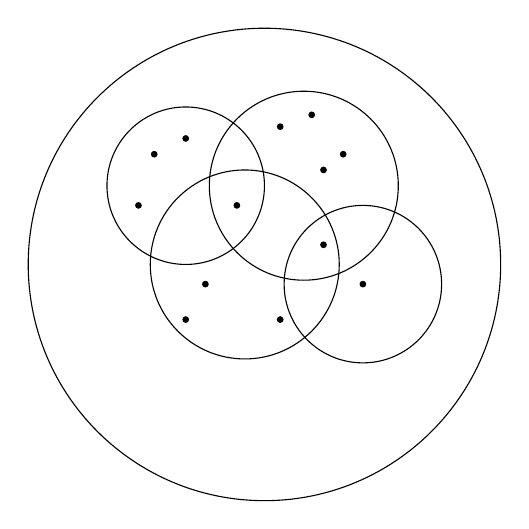
\begin{tikzpicture}[point/.style={draw,circle,inner sep=0cm,fill=black,minimum size=2pt}]
        \draw (0,0) circle [radius=3cm];
        \draw (-1,1) circle [radius=1cm];
        \draw (-0.25,0) circle [radius=1.2cm];
        \draw (0.5,1) circle [radius=1.2cm];
        \draw (1.25,-0.25) circle [radius=1cm];
        \node[point] () at (-1.4,1.4) {};
        \node[point] () at (-1,1.6) {};
        \node[point] () at (-1.6,0.75) {};
        \node[point] () at (-0.35,0.75) {};
        \node[point] () at (0.2,1.75) {};
        \node[point] () at (0.6,1.9) {};
        \node[point] () at (1,1.4) {};
        \node[point] () at (0.75,1.2) {};
        \node[point] () at (0.75,0.25) {};
        \node[point] () at (1.25,-0.25) {};
        \node[point] () at (-0.75,-0.25) {};
        \node[point] () at (-1,-0.7) {};
        \node[point] () at (0.2,-0.7) {};
    \end{tikzpicture}
\end{document}
